\chapter{Modèles}

\section{Choix des modèles}
Le choix des modèles a été un choix rapide.\newline
Nous avons commencé par regarder les tutoriels sur les sites web des frameworks que nous utilisons. Nous avons donc regardé les tutotiels de pytorch, car nous voulions utiliser ce framework en particulier, mais avons aussi regardé les githubs de modèles dont nous avions entendu parler, comme YOLOv5. Il faut noter que notre compréhension du problème et du jargon utilisé dans le domaine s’est enrichi au fur et à mesure de nos recherches. \newline 
Ainsi, nos premiers choix peuvent sembler mauvais, mais lors de la prise de décision nous étions persuadés de faire les bons choix. Notre approche de départ se basait essentiellement sur un facteur: nous voulions des modèles pour lesquels il existe beaucoup de ressources en ligne. Cette méthodologie nous a amené à explorer une solution (YOLOv5) qui n’était pas adaptée à notre problème. \newline
Après beaucoup d’essais infructueux, nous avons donc changé de méthodologie et nous nous sommes laissé la liberté d’utiliser des outils de plus haut niveau, tel que Detectron2 et de ne pas se restreindre uniquement à PyTorch. Une fois que nous avons pris en main ce framework, nous avons pu nous concentrer sur la performance du modèle. C'est aussi à ce stade que nous avons compris que le score sur le benchmark COCO2017 indiqué sur beaucoup de documentation de modèles était justement indiqué pour pouvoir comparer les modèles entre eux.

\section{Les échecs}
\subsubsection{YOLOv5}
YOLO est l'acronyme de You Only Look Once; il s'agit du premier modèle que nous avons essayé. Nous avons décidé de commencer avec ce modèle pour plusieurs raisons parmi lesquelles : une abondance de tutoriels sur le net et une solution qui nous semblait clé en main pour résoudre notre problème. Malgré ces signes positifs, il n’a pas été une solution adaptée. \newline
En effet, YOLO, a été publié il y a plusieurs année et n’est plus forcément l’état de l’art actuel. De plus, ce modèle est adapté à du traitement en temps réel ce qui ne fait pas partie de notre problème. Cependant, le réel souci qui nous a fait abandonner cette solution est la structure spéciale du dataset qui ne correspondait pas à notre structure. \newline 
Durant une phase de réflexion visant à résoudre le souci de structure, nous avons ainsi réalisé l’incapacité du modèle à gérer des images n’étant pas de 640x640 pixels. Nous aurions pu effectuer un réajustement de la taille des images mais ces derniers éléments nous ont fait réaliser que YOLO n’était pas la solution clé à laquelle nous nous attendions et avons décidé après quelques discussions de passer à un modèle plus adapté à notre problème initial. C'est ainsi que nous nous sommes lancé sur faster R-CNN, un modèle qui supporte des images de tailles arbitraires et qui est plus récent que YOLOv5.

\subsubsection{SSD}

\subsubsection{Faster RCNN avec Keras}


\section{FASTER R-CNN}

source1 : https://towardsdatascience.com/r-cnn-fast-r-cnn-faster-r-cnn-yolo-object-detection-algorithms-36d53571365e \newline\newline
source2 : https://stackoverflow.com/questions/48318448/understanding-basic-difference-between-a-cnn-and-rnn \newline\newline
+ check videos en cherchant "rcnn, fast rcnn, faster rcnn" sur google






\paragraph{Description}





\begin{itemize}
    \item Histoire (evolution de RCNN) 
    \item Date du papier l’expliquant 
    \item architecture
    \item Score benchmark coco
\end{itemize}
Adapter les exemples sur un problèmes légèrement différent : bullshiter sur assembler différent tutoriaux nécessite de comprendre, perte de temps sur manque de connaissance du jargon technique : mAP, etc les benchmarks coco, comprendre que coco (Common Object in COntext) est beaucoup de chose (dataset, benchmark baseline, dataset d’entrainement)





\section{RETINA net}
\paragraph{Description}

\paragraph{Results}








\section{DEtection Transformer (DE-TR)}
\paragraph{} 
\href{https://github.com/facebookresearch/detr}{DETR} est un modèle sorti en 2020 qui est extrêmement simple à implémenter et fournit des scores (mAP, IoU etc) sur le dataset COCO qui surpassent ceux des modèles existants de quelques points. C’est pourquoi, en plus de son architecture innovante, nous avons voulu l’essayer. L’architecture, visible en figure \ref{fig:detr_architecture}, se base sur un transformer, un modèle de deep learning parut dans le fameux papier de 2017 de Google, \href{https://arxiv.org/pdf/1706.03762.pdf}{\textit{Attention is all you need}}. On peut observer que le modèle commence par génèrer des features à partir de l'image d'entrée en utilisant une backbone c'est à dire un modèle pré-entrainé visant justement à extraire ces features à l'aide d'un réseau convolutionnel. Ensuite, le modèle utilise la partie encodeur du transformer suivit du décodeur et finalement d'un \verb|prediction feed-forward networks| (FFN). C'est le réseau FFN qui génère les possibles boundings boxes et les classes associées.

\begin{figure}[th!]
    \centering
    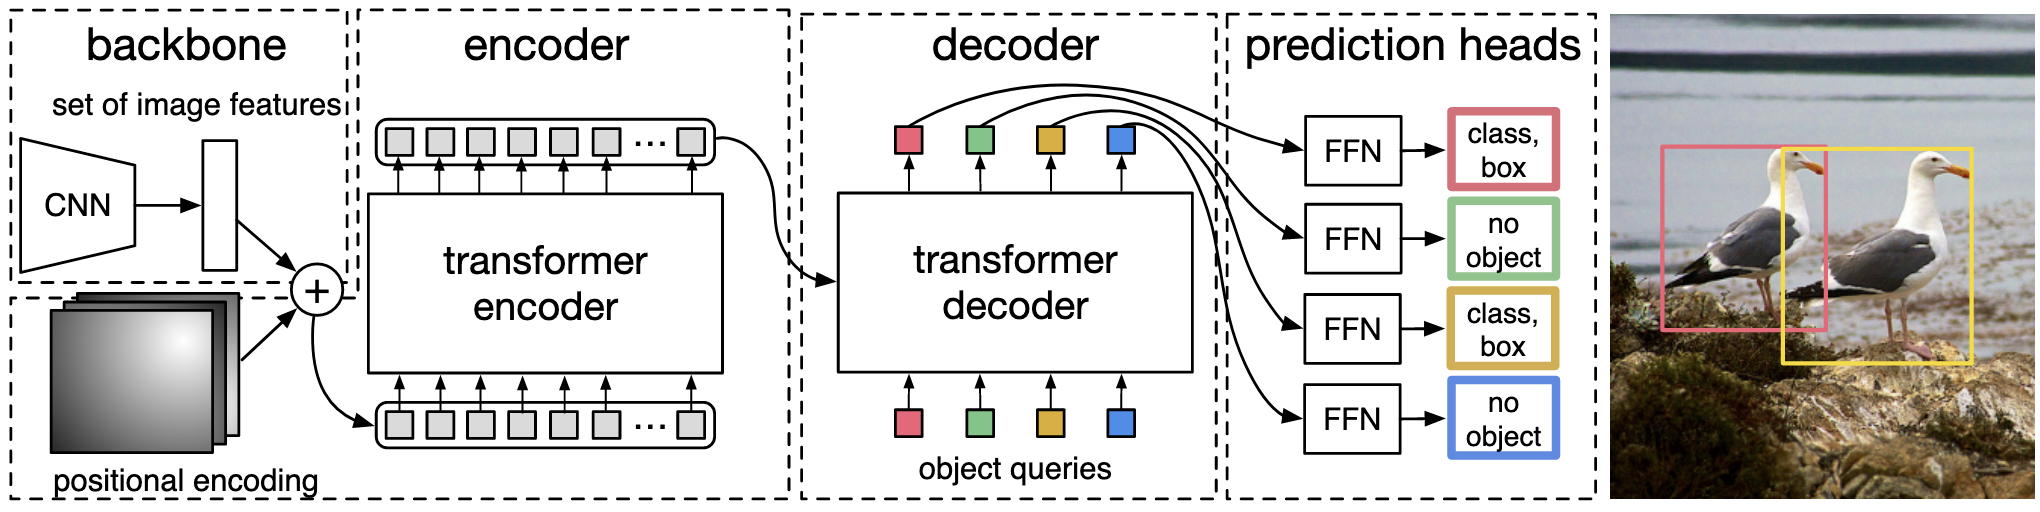
\includegraphics[width=\textwidth]{images/detr_architecture.png}
    \caption{Architecture de DETR}
    \label{fig:detr_architecture}
\end{figure}
% ----------------------------------------------------
